%第3章



\section{基本設計}

問題領域やシステムの構造を論理的,静的にみるためにクラス図を作成した.以下に図\ref{class_ic}を載せる.

\begin{figure}[htbp]
\centering
\includegraphics[width=15cm]{./picture/class_ic.eps}
\caption{ICタグを用いたシステムのクラス図}
\label{class_ic}
\end{figure}

\begin{figure}[htbp]
\centering
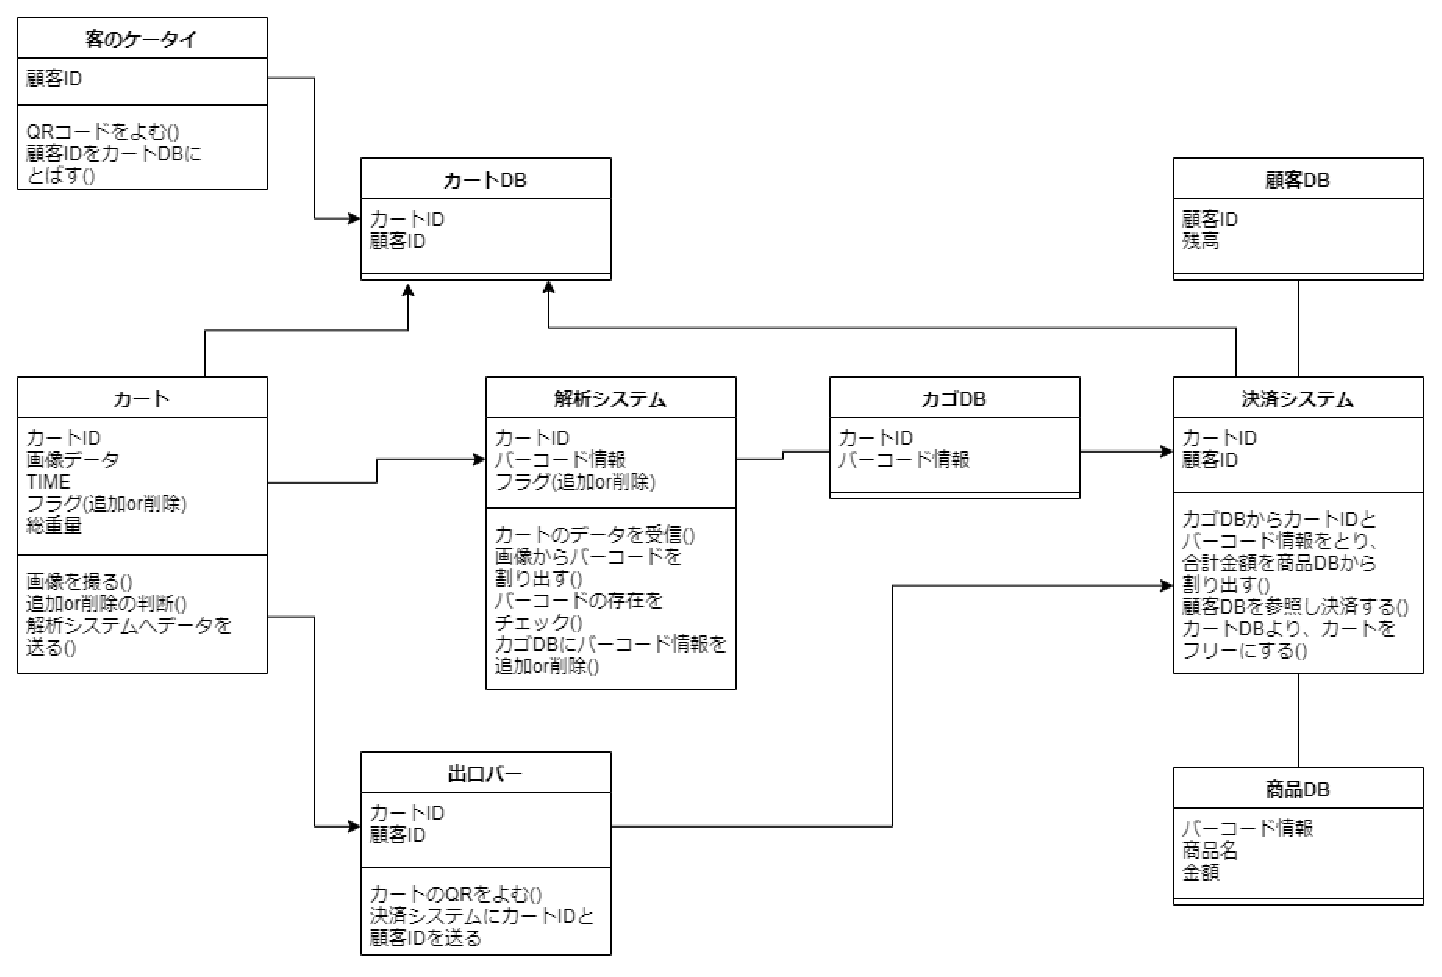
\includegraphics[width=15cm]{./picture/class_qr.eps}
\caption{QRコードを用いたシステムのクラス図}
\label{class_qr}
\end{figure}

\begin{figure}[htbp]
\centering
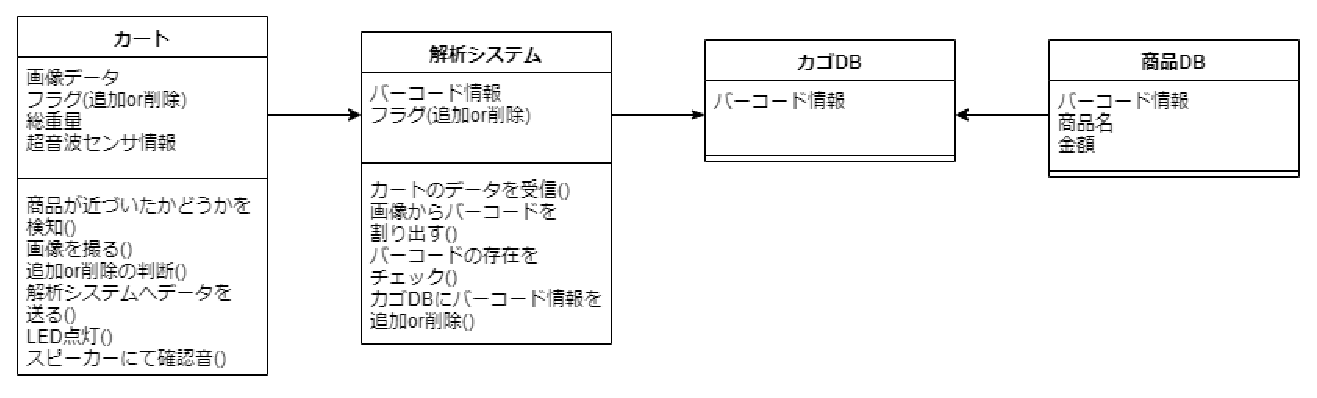
\includegraphics[width=15cm]{./picture/class_qr_2.eps}
\caption{実装するシステムのクラス図}
\label{class_qr_2}
\end{figure}